\documentclass[
../../NLP4W_Summary.tex,
]
{subfiles}
    
\externaldocument[ext:]{../../NLP4W_Summary.tex}
% Set Graphics Path, so pictures load correctly
\graphicspath{{../../}}

\begin{document}
\section{Information Retrieval 1}
Information Retrieval concerns itself with how we can get relevant information from a corpus of data.

\begin{defbox}
    [Relevant Terms for Information Retrieval]
    \begin{itemize}
        \item Document: Can be anything (web page, word file, text file, article, etc.)
        \item Collection: A set of documents (Assumed static for now, makes it easier to use)
        \item Query: Piece of information that is searched for
        \item Relevance: Whether a document satisfies the information need of the user.
        \begin{itemize}
            \item Relevance often measured by how often a term appears in a document.
            \item This needs to be in conjunction with the length of the document, as the longer a document is the more likely it is to contain the relevant query more often.
            \item However, this counting approach gets inefficient for queries.
        \end{itemize}
    \end{itemize}
\end{defbox}

\subsection{Inverted Index}
The Inverted Index is a method of efficiently retrieving documents from large collections.
Hereby the inverted index stores all statistics that the scoring model needs per term, such as:
\begin{itemize}
    \item Document frequency: How many documents contain the term
    \item Term frequency per document: How often the term appears in the document
    \item Document length: Length of the document
    \item Average document length: Average length of all documents
\end{itemize} 
These statistics are saved in a format that is accessible by a given term. Also saves metadata of the documents (Name, location, etc.)

\begin{minipage}[t]
    {0.37\textwidth}
    \begin{defbox}
        [Inverted Index Structure]
        \begin{center}
            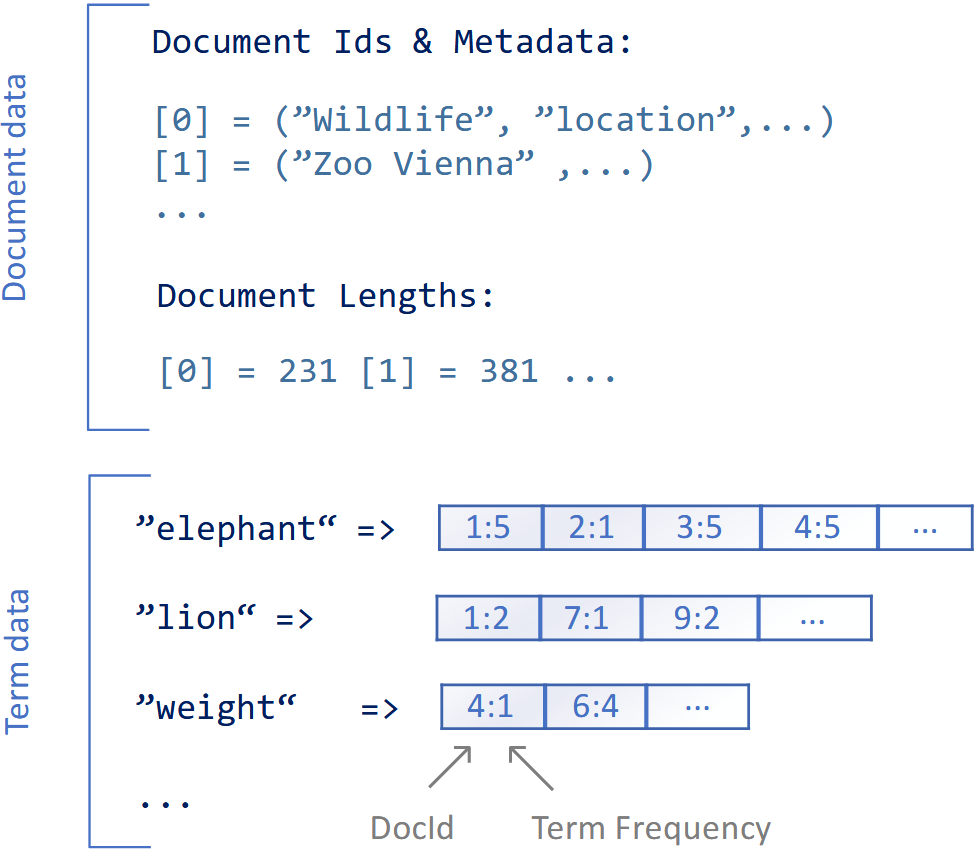
\includegraphics[width=\textwidth]{Pics/InvertedIndexStructure.png}
        \end{center}

        \begin{itemize}
            \item Every document has internal document ID
            \item Term dictionary is saved as search friendly data structure (dictionary (HashMap))
            \item Term frequencies are stored in a "posting list" of doc ids and frequency pairs\\
            $\rightarrow$ not good for random lookups
        \end{itemize}
    \end{defbox}
\end{minipage}
\hfill
\begin{minipage}
    [t]{0.63\textwidth}
    \begin{defbox}
        [Inverted Index Creation]
        \begin{center}
            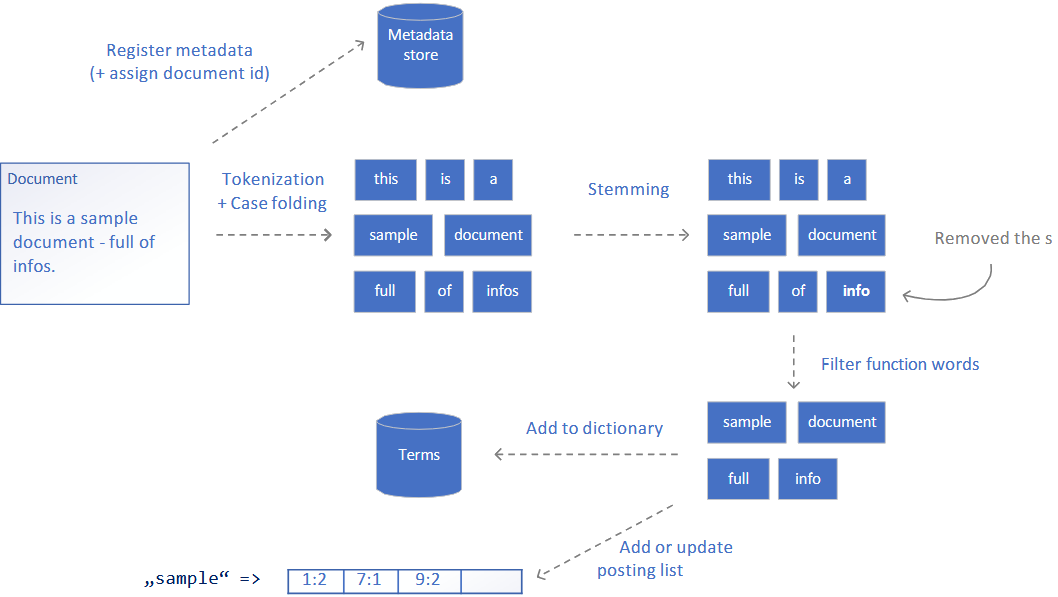
\includegraphics[width=\textwidth]{Pics/InvertedIndexCreation.png}
        \end{center}
        
        \begin{itemize}
            \item Linguistic models are language dependent
            \item A query text and a document text undergo the same process
        \end{itemize}
    \end{defbox}
\end{minipage}

\begin{defbox}
    [Inverted Index Querying]
    \begin{center}
        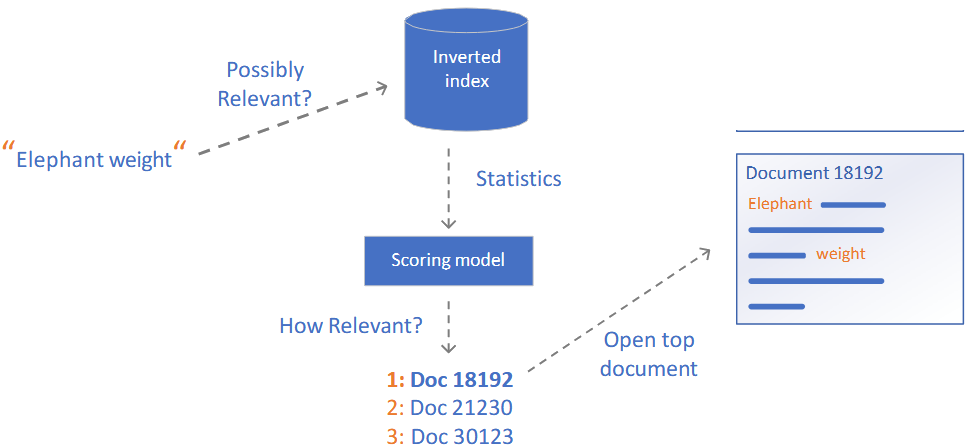
\includegraphics[scale=0.4]{Pics/InvertedIndexQuerying.png}
    \end{center}
    \begin{itemize}
        \item No need to read full documents
        \item Only operates on frequency numbers of potentially relevant documents 
        \item Sort documents based on relavance
    \end{itemize}
\end{defbox}

\subsection{Search \& Relevance}
\begin{defbox}
    [Types of queries]
    A query can take many forms, for example:
    \begin{itemize}
        \item Exact matching: Document needs to contain the query exactly
        \item Boolean queries: Uses logical operators (AND, OR, NOT) to combine queries
        \item Expanded queries: Incorporates synonyms and other relevant words into the query
        \item etc.
    \end{itemize}
    Queries do not have to be in text form, they can also be sound/phonetic (e.g. Music recognition, speech recognition), images (e.g. Image search), etc.
    We do focus on text queries for now.
\end{defbox}

Every search is based on how relevant the documents are to the query. Hereby we use a scoring model that takes inputs from the document and the query and outputs a relevance score (floating point value).

A simple search algorithm utilizing the inverted index is:

\begin{codebox}[Search Algorithm]
    \begin{algorithm}[H]
        \SetKwFunction{search}{search}
        \Fn{\search{query, k}}{
            \KwFloat[] scores = $\emptyset$\;
            \ForEach{query term q \KwIn query}{
                Fetch term data tf for q\;
                \ForEach{pair(d, tf$_{t,d}$ in term data)}{
                    \If{d \KwNot \KwIn scores}{
                        scores[d] = 0\;
                    }
                    scores[d] += score(d, tf$_{t,d}$)\;
                }
            }
            \KwRet k biggest entries of scores\;
        }
    \end{algorithm}
\end{codebox}

\begin{defbox}
    [Relevance Scoring]
    \begin{itemize}
        \item Relevance scoring is usually based on word occurences
        \item Simply counting how often a term appears in a document is not enough as it does not take into account the length of the document
        \item Therefore, we need to adjust the scoring accordingly.
        \item Relevance is often assumed to be binary. This means that a document is either relevant or not, no partials.
        \item Relevancy is too complex, therefore we need oversimplifications to create and evaluate mathematical models.
    \end{itemize}
\end{defbox}

\subsection{Term Frequency \& Document Frequency Models}
\subsubsection{Term Frequency}
Term frequency is the number of times a term appears in a document. Often denoted as $tf_{t,d}$, how often term t appears in document d. However, often relative frequencies make more sense to use than absolute frequencies (See above). Retrieval experiments show that logarithm of term frequency works well for this.
\begin{figure}
    [htp]
    \centering
    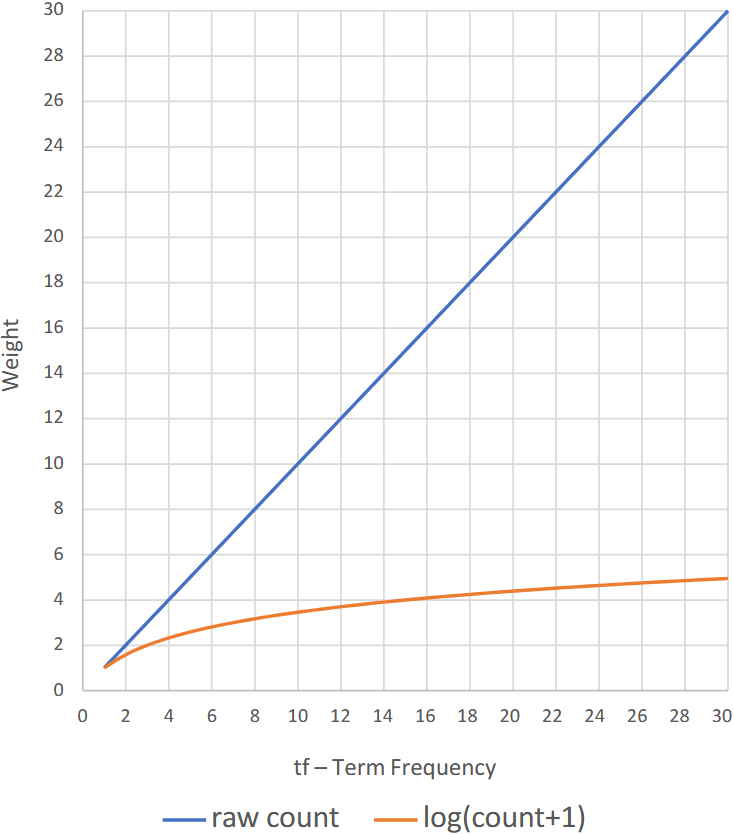
\includegraphics[scale=0.4]{Pics/AbsoluteVSRelativeFrequency.png}
\end{figure}

\subsubsection{Document Frequency}
The document frequency is the number of documents that contain a term. Often denoted as $df_t$.
Here rare terms are more informative than frequent terms (like function words: the, or, a, etc.)
Therefore for our frequency we want a high weight for rare terms.

\begin{defbox}
    [IDF - Inverse Document Frequency]
    The common way to define the inverse document frequency of a term: 
    \begin{center}
        \begin{smallmathbox*}
            \shortstack{
                $idf(t) = \log (\dfrac{|D|}{df_t})$\\
                with total number of documents $|D|$ and number of documents with $tf_t > 0$ $df_t$ 
            }
        \end{smallmathbox*}
    \end{center}
    It describes how common the term is in the corpus. The higher the $idf$ the more common the term is.
\end{defbox}

\begin{defbox}
    [TF-IDF]
    The TF-IDF is a combination of term frequency and inverse document frequency:
    \begin{center}
        \begin{smallmathbox*}
            \shortstack{
                $TF\_IDF(q,d) = \sum\limits_{t \in T_d \cap T_q} \underbrace{\log (1+ tf_{t,d})}_{*1} \cdot \underbrace{\log (\dfrac{|D|}{df_t})}_{*2}$\\
                with query $q$, document $d$, term frequency $tf_{t,d}$, total number of documents $|D|$, \\
                and number of documents with $tf_t > 0$ $df_t$\\
                $*1$: increases with the occurences of the term in the document\\
                $*2$: increases with the rarity of the term in the collection
            }
        \end{smallmathbox*}
    \end{center}
    A rare word in the collection appearing a lot in one document creates a high score, while common words are downgraded.

    TF-IDF is not only useful in document retrieval. The weights can also be used as a base for other retrieval models and also for generic word weighting mechanism for NLP
\end{defbox}

\begin{defbox}
    [BM25]
    BM25 is an extension of TF-IDF. 

    \begin{center}
        \begin{smallmathbox*}
            \shortstack{
                $BM25(q,d) = \sum\limits_{t \in T_d \cap T_q} \dfrac{tf_{t,d}}{k_1((1-b) + b \dfrac{dl_d}{\text{avgdl}}) + tf_{t,f}} \cdot \log \dfrac{|D| - df_t + 0.5}{df_t + 0.5}$ \\
                with query $q$, document $d$, term frequency $tf_{t,d}$, document length $dl_d$,\\ average document length $\text{avgdl}$, total number of documents $|D|$,\\ number of documents with $tf_t > 0$ $df_t$ and hyperparameters $k_1$ and $b$
            }
        \end{smallmathbox*}
    \end{center}
    The hyperparameters $k_1$ and $b$ are set by the user. Hereby $k_1$ controls the term frequency scaling ($k_1 = 0$ is a binary model, large $k_1$ is raw term frequency).
    $b$ controls document length normalization ($b = 0$ is no normalization; $b = 1$ is relative frequency (full scale by document length)).
    Common ranges: $0.5 < b < 0.8$ and $1.2 < k_1 < 2$.
\end{defbox}

\begin{figure}
    [htp]
    \centering
    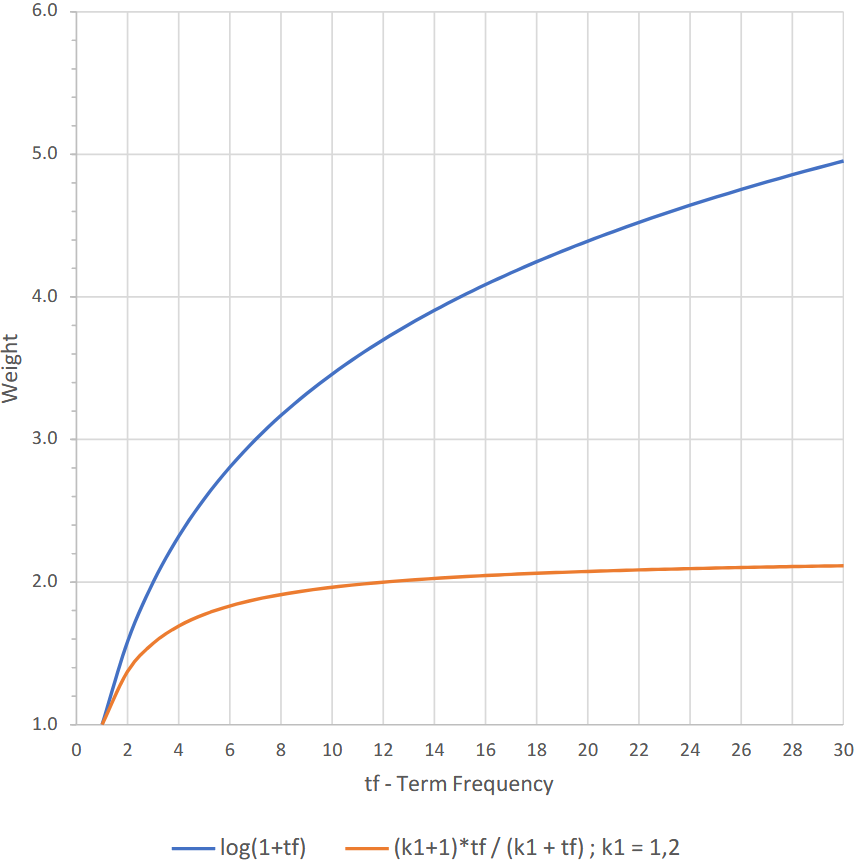
\includegraphics[scale=0.35]{Pics/TFIDFVSBM25.png}
    \caption{TF-IDF alwasy increases, while BM25 asymptotes at $k_1 + 1$}
\end{figure}

\newpage
\subsection{Evaluation}
The evaluation of systems is done by observing concrete evidence for a hypothesis. It is compared to other systems on performance.

Performance can be different things depending on context:
\begin{itemize}
    \item Result quality: Are the results correct / as expected?
    \item Efficieny: How fast is the system?
    \item Fairness, diversity, content quality, source credibility, effort, etc.
    \item Retrieval of Context of a Larger Goal:
    \begin{itemize}
        \item How big is the scope of the system?
        \item How well does it integrate with the web?
    \end{itemize}
\end{itemize}

Information Retrieval Systems are hard to evaluate, due to their ambiguity (what is relavance, context, etc.) and collection size (The more the size of the collection differs from one system to another, the more the evalutation setting differs from each other).

In general there are two types of evaluation:
\begin{itemize}
    \item \textbf{Intrinsic:} Fixed set, same collection, query and labels
    \item \textbf{Extrinsic:} Observe behaviour of users
\end{itemize}

\begin{defbox}
    [Extrinsic Evaluation Setup]
    \begin{itemize}
        \item Considers the quality of systems that produce a ranked list of documents.
        \item Compared to a (predefined, desired) pool of judgements (not necessarily the whole list)
        \item Missing judgements are often considered as non-relevant
    \end{itemize}
    \begin{center}
        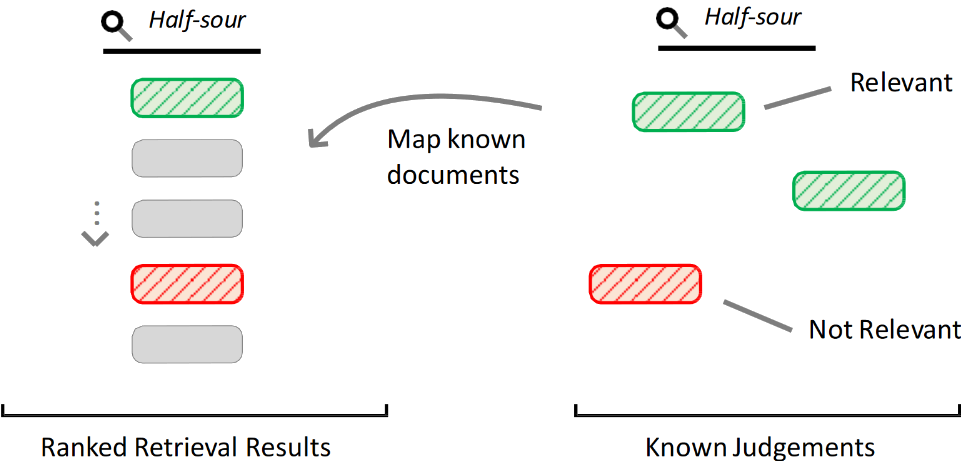
\includegraphics[scale=0.5]{Pics/ExtrinsicEvaluationScheme.png}
    \end{center}
    Using this scheme we can evaluate and compare systems on how well they rank documents.
\end{defbox}

\subsubsection{Precision \& Recall}
\begin{figure}
    [htp]
    \centering
    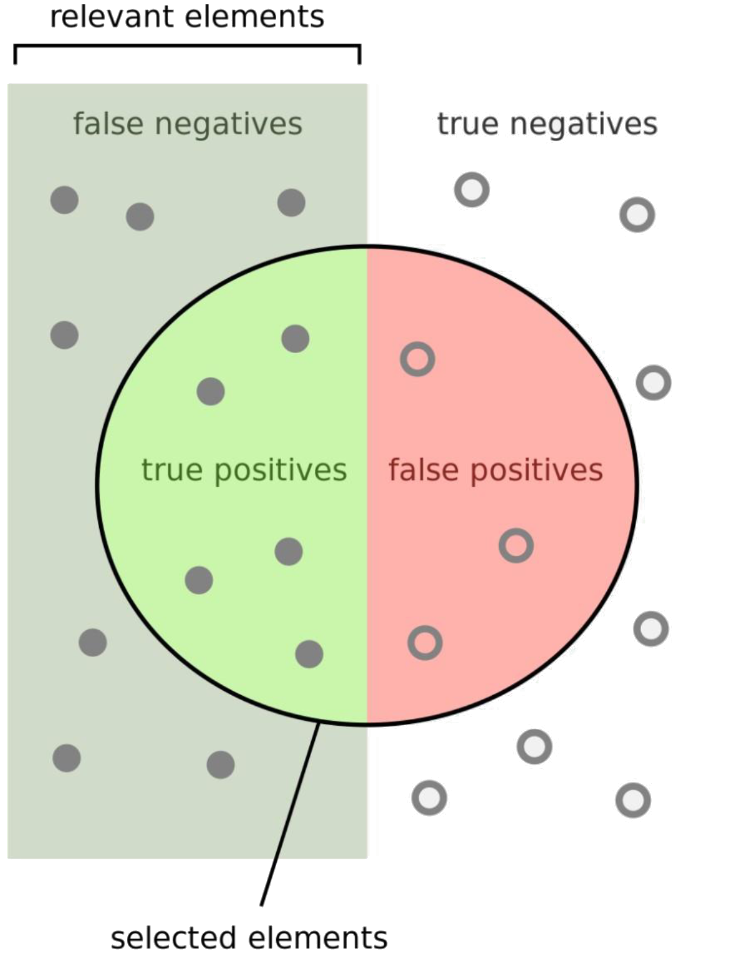
\includegraphics[scale=0.3]{Pics/RetrievedDocuments.png}
\end{figure}

Precision and Recall are both metrics which can be used to compare a systems performance on.

\begin{minipage}
    [t]{0.45\textwidth}
    \begin{center}
        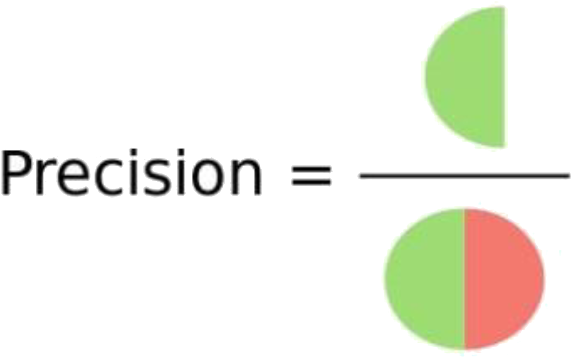
\includegraphics[width=0.4\textwidth]{Pics/Precision.png}
    \end{center}

    Hereby \textbf{Precision} is the ratio of relevant documents found to the total number of documents found.
\end{minipage}
\hfill
\begin{minipage}
    [t]{0.45\textwidth}
    \begin{center}
        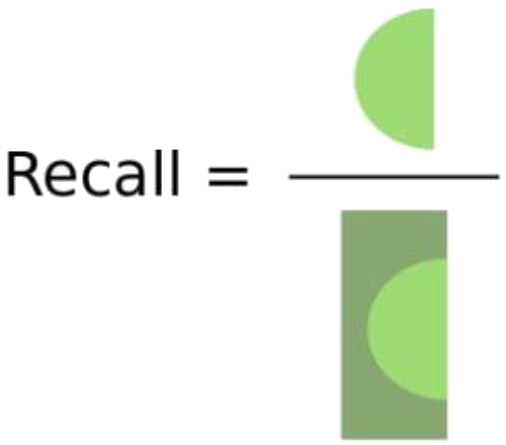
\includegraphics[width=0.4\textwidth]{Pics/Recall.png} 
    \end{center}
    
    \textbf{Recall} is the ratio of relevant documents found to the total number of relevant documents.
\end{minipage}
\vspace{10pt}

Building a model that increases recall or precision is fairly easy. 

If a system needs less certainty to return a document it'll return more documents total. This means that it'll be more likely to return more relevant documents, but also more irrelevant documents. Since Recall is not dependent on the irrelevant documents, it'll increase Recall (This also means that a system that returns all documents will have 100\% Recall). The oposite is true for precision, if you increase the certainty needed to return a document it'll increase the precision, but it'll also miss more relevant documents.

\newpage
Due to this we often measure performance as the combined measure \textbf{F-Score}.
It's mostly used as $F_1$, which describes the harmonic mean of P and R: 

\begin{center}
    \begin{smallmathbox*}
        $F_1 = 2 \times \dfrac{P \times R}{P + R}$
    \end{smallmathbox*}
\end{center}

So in general the forms look like this:
\begin{table}[htp]
    \centering
    \begin{tabular}{|l|l|l|l|l|}
        \hline
        & \textbf{Relevant} & \textbf{Non-Relevant} \\ \hline
        \textbf{Retrieved} & TP (True Positive) & FP (False Positive) \\ \hline
        \textbf{Not Retrieved} & FN (False Negative) & TN (True Negative) \\ \hline
    \end{tabular}
\end{table}

\begin{minipage}
    [t]{0.3\textwidth}
    \begin{center}
        \begin{smallmathbox}
            [Precision]
            $P = \dfrac{TP}{TP + FP}$
        \end{smallmathbox}
    \end{center}
\end{minipage}
\hfill
\begin{minipage}
    [t]{0.3\textwidth}
    \begin{center}
        \begin{smallmathbox}
            [Recall]
            $R = \dfrac{TP}{TP + FN}$
        \end{smallmathbox}
    \end{center}
\end{minipage}
\hfill
\begin{minipage}
    [t]{0.3\textwidth}
    \begin{center}
        \begin{smallmathbox}
            [F-Score]
            $F_1 = \dfrac{2 \times P \times R}{P + R}$
        \end{smallmathbox}
    \end{center}
\end{minipage}

\newpage
\subsection{MRR \& MAP}
The MRR (Mean Reciprocal Rank) and MAP (Mean Average Precision) are metrics that can be used to evaluate the performance of a system. Using these we can devise a way to rank and compare the retrieval of documents of systems. 

Usually these are measured over all retrieved documents but only over the top @k retrieved documents. For MAP / Recall higher numbers like @100 or @1000 are used, while MRR / Precision are more likely to be smaller like @5 or @10.

\subsubsection{MRR}
\begin{defbox}
    [MRR: Mean Reciprocal Rank]
    The MRR basically looks at ranking from the perspective of a single query. It can be seen as the solution for a user that only cares about the first relevant document and doesn't care about any others. 
    \begin{center}
        \begin{smallmathbox*}
            \shortstack
            {MRR($Q$) $= \underbrace{\dfrac{1}{|Q|}}_{\text{MQ}} \cdot \sum\limits_{q \in Q} \underbrace{\dfrac{1}{\text{FirstRank}(q)}}_{\text{RR}}$\\
            with Query Set $Q$ and FirstRank($q$) returning the first relevant document for the query\\
            where MQ is the Mean over all queries and RR is the Reciprocal Rank}
        \end{smallmathbox*}
        Hereby a higher result indicates a better model.
    \end{center}

    The MRR is applicable with sparse judgements or assuming users are satisfied with one relevant document.
\end{defbox}

\begin{figure}
    [htp]
    \centering
    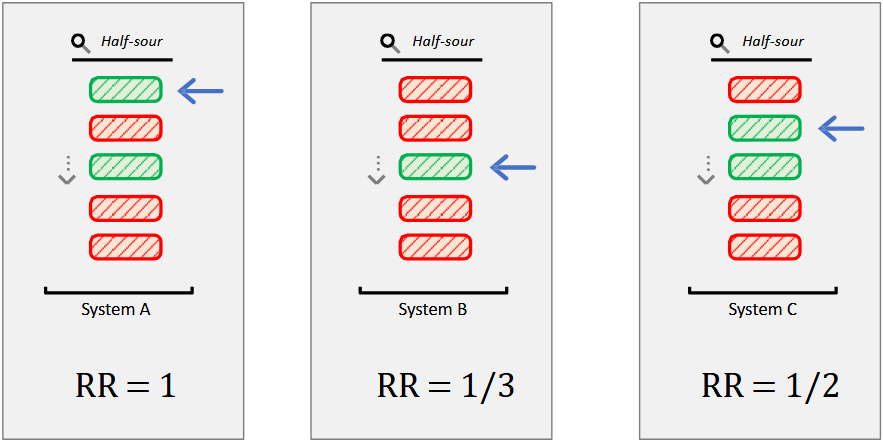
\includegraphics[width=0.6\textwidth]{Pics/MRRExample.png}
    \caption{Reciprocal Rank Example}
\end{figure}

\begin{figure}
    [htp]
    \centering
    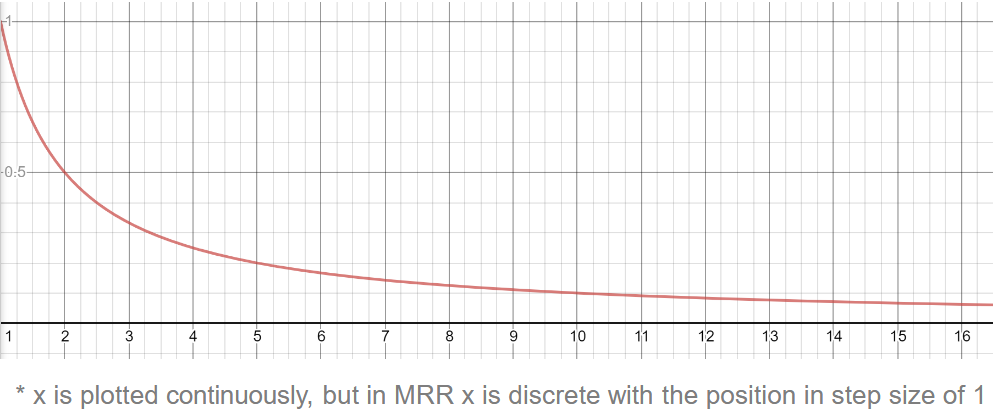
\includegraphics[width=0.7\textwidth]{Pics/MRRPlot.png}
    \caption{Reciprocal Rank Progression}
\end{figure}


\subsubsection{MAP}
\begin{defbox}
    [MAP: Mean Average Precision]
    The MAP responds to the area under the Precision-Recall curve.
    \begin{center}
        \begin{smallmathbox*}
            \shortstack{
                MAP($Q$) $= \underbrace{\dfrac{1}{|Q|}}_{\text{MQ}} \cdot \sum\limits_{q \in Q} \dfrac{\overbrace{\sum_{i=1}^{k} P(q)_{@i} \cdot \text{rel}(q)}^{\text{PRD}}}{\underbrace{|\text{rel}(q)|}_{\text{AP}}}$\\
                with Query Set $Q$, Precision of query after the first $i$ documents,\\ relevance of doc at position $i$ rel$(q)$, number of relevant documents |rel$(q)$|\\
                where MQ is the mean over all queries,\\ PRD is the Precision per relevant doc and AP is the Average Precision
            }
        \end{smallmathbox*}
        k describes the first k results of a system and can be chosen accoding to the needs. The number of relevant docs is also defined beforehand by the annotators.
    \end{center}
    This metric also considers the relevance and order of the documents in the ranking.
\end{defbox}

\begin{figure}
    [htp]
    \centering
    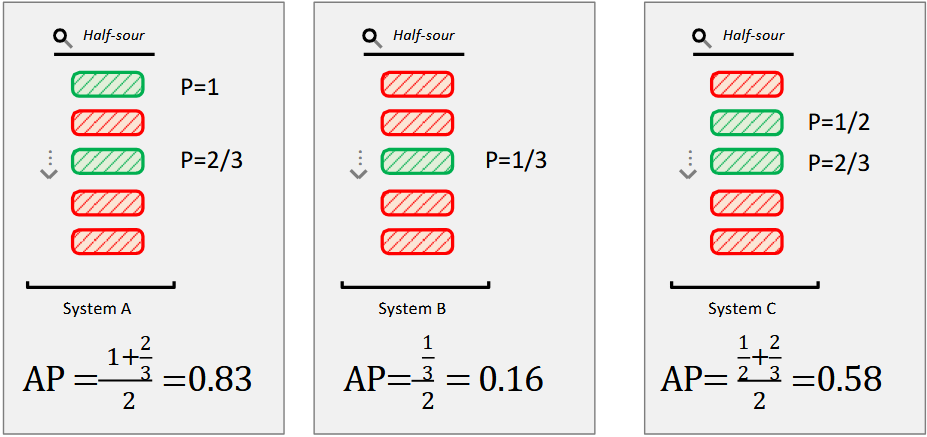
\includegraphics[width=0.6\textwidth]{Pics/MAPExample.png}
    \caption{Average Precision Example}
\end{figure}

\subsection{nDCG}

The normalized Discounted Cumulative Gain (nDCG) is another metric for ranking list evaluation. 
Hereby it differs from MRR and MAP because it uses graded relevance. MRR and MAP used Binary, meaning that in the model a document could either be relavant or not relevant. 

nDCG works with graded relevance, meaning that a relevant document can be less or more relevant than another relevant document. 

\begin{defbox}
    [Common Graded Relevance Labels]
    \begin{itemize}
        \item[[  3]] Perfectly relevant: Dedicated to the query, worthy of being a top result
        \item[[  2]] Highly relevant: Provides substantial information on the query
        \item[[  1]] Relevant: Provides some information on the query, may be minimal
        \item[[  0]] Irrelevant: Provides no information on the query
    \end{itemize}
    Relevance can also be defined otherwise. Another common approach is to use a floating point value instead of a label.
\end{defbox}

\begin{defbox}
    [nDCG: normalized Discounted Cumulative Gain]
    \begin{center}
        \begin{smallmathbox*}
            \shortstack{
                DCG$(D) = \sum\limits_{d \in D,\space i = 1} \dfrac{\text{rel}(d)}{\log_2(i+1)}$\\
                with single document results list $D$ and relevance grade for query-doc pair rel$(d)$
            }
        \end{smallmathbox*}

        \begin{smallmathbox*}
            \shortstack{
                nDCG$(Q) = \dfrac{1}{|Q|} \cdot \sum\limits_{q \in Q} \dfrac{\overbrace{\text{DCG}(q)}^{\text{Actual Result}}}{\underbrace{\text{DCG}(\text{sorted}(q))}_{\text{Best Possible Result}}}$\\
                with Query Set $Q$ and sorted list of relevance grades for a query $\text{sorted(rel}(q))$
            }
        \end{smallmathbox*}
    \end{center}
\end{defbox}

\begin{figure}
    [htp]
    \centering
    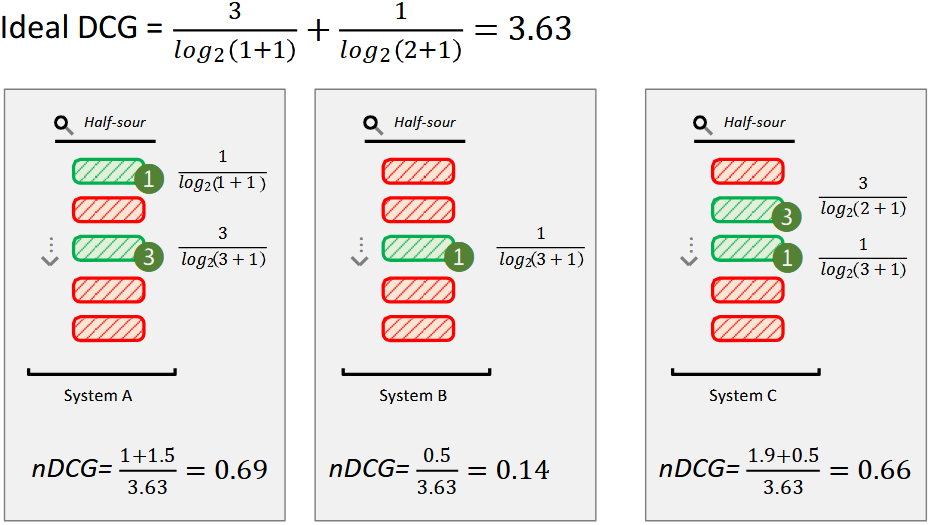
\includegraphics[width=0.6\textwidth]{Pics/DCGExample.png}
    \caption{DCG Example}
\end{figure}

\begin{figure}
    [htp]
    \centering
    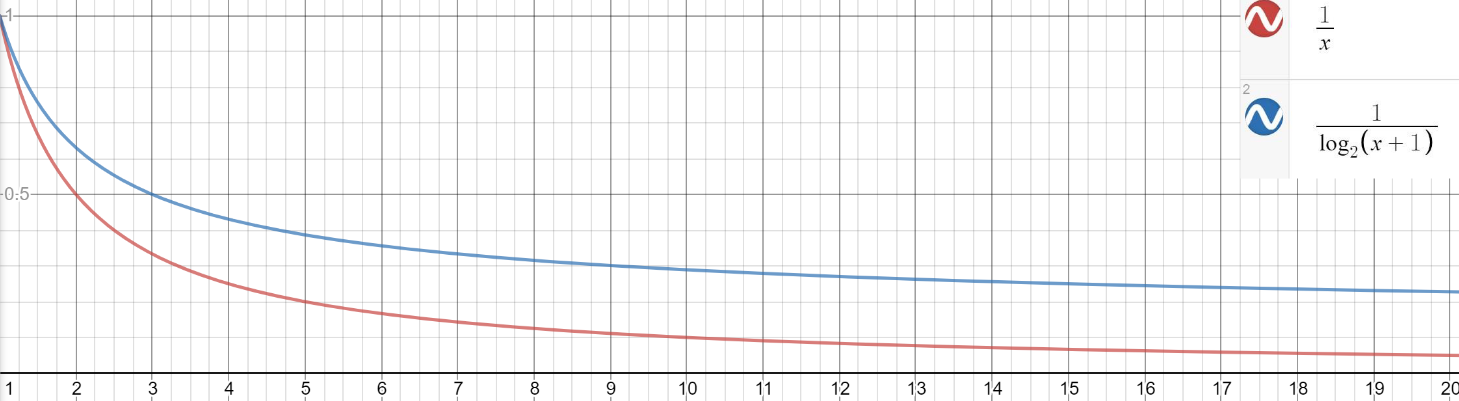
\includegraphics[width=0.8\textwidth]{Pics/DCGVsRR.png}
    \caption{DCG vs. RR}
\end{figure}
\end{document}